%/*****************************************************************************
% * Download Elevation File
%/*****************************************************************************

\documentclass[12pt]{article}
\usepackage{float}
\usepackage{graphicx}
\usepackage[margin=1in]{geometry}

\graphicspath{{images/}}

\usepackage[utf8]{inputenc}
\usepackage[english]{babel}
\usepackage[parfill]{parskip}
\usepackage{datetime}
\usepackage{hyperref}
\hypersetup{
	colorlinks=true,
	urlcolor=blue,
  }
\urlstyle{same}
\usepackage{subcaption} 
\usepackage{dirtytalk}
\usepackage{multirow}
\usepackage{booktabs}


\usepackage{fancyhdr}
\pagestyle{fancy}
\fancyhf{}
\rhead{How to download an elevation file using WindNinja}
\cfoot{\thepage}

\newcommand\vn{3.6.0}

\begin{document}
\begin{titlepage}
    \centering
    {\Huge
       How to download an elevation file using WindNinja
    }    
    \vfill
    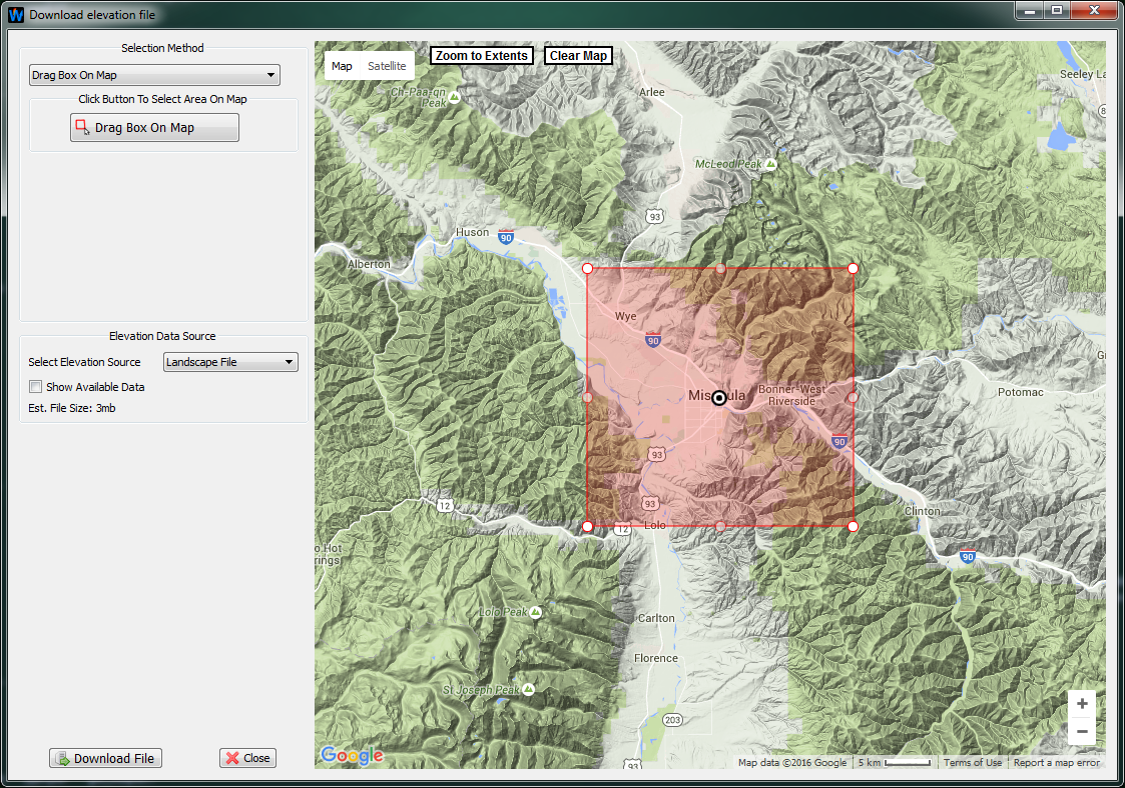
\includegraphics[scale=0.75]{dem_download_0}
    \vfill
  	{\Huge
	  6/30/2023 %Date Last Edited
  	}
    \vfill
\end{titlepage}


\section*{Introduction}
This document describes the functionality built into WindNinja to download
elevation files for wind modeling.  We call this utility the “elevation file
grabber”.  It allows you to use a custom \textcopyright Mapbox \textcopyright OpenStreetMap interface to zoom into
and select a desired area for wind modeling. The elevation data for this area
is downloaded by WindNinja from a USGS server and saved to a file on your
computer.  There is also a command line version of the elevation file grabber
that is described \href{https://weather.firelab.org/windninja/tutorials/fetch_dem_instructions.pdf}{here}.  The specific
options available and work flow are described below.

To open the elevation file grabber window, start WindNinja and click \textit{Surface Input} in the navigation tree at the top of WindNinja, then click the \textit{Download File} button as shown below.

\begin{figure}[H]
	\centering
	\label{}
	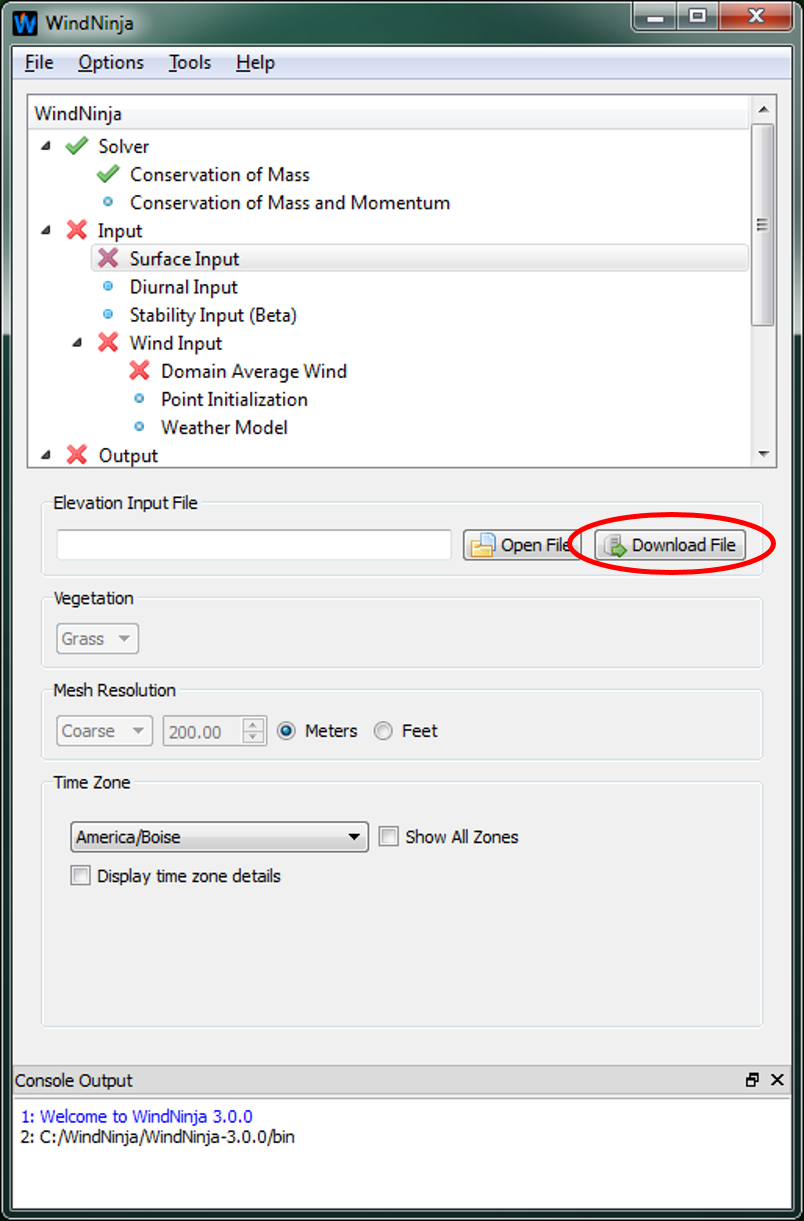
\includegraphics[scale=0.75]{main_window_0}
\end{figure}
\newpage

The \textit{Download Elevation File} graphics window will open. This graphics window is an interactive mapping display used to navigate into the desired wind simulation area. There are a couple of ways to pan and zoom the map.  Using a mouse, you can pan with the left button and zoom using a mouse scroll wheel.  The keyboard can also be used to pan (arrow keys) and zoom (plus and minus keys).

\begin{figure}[H]
	\centering
	\label{}
	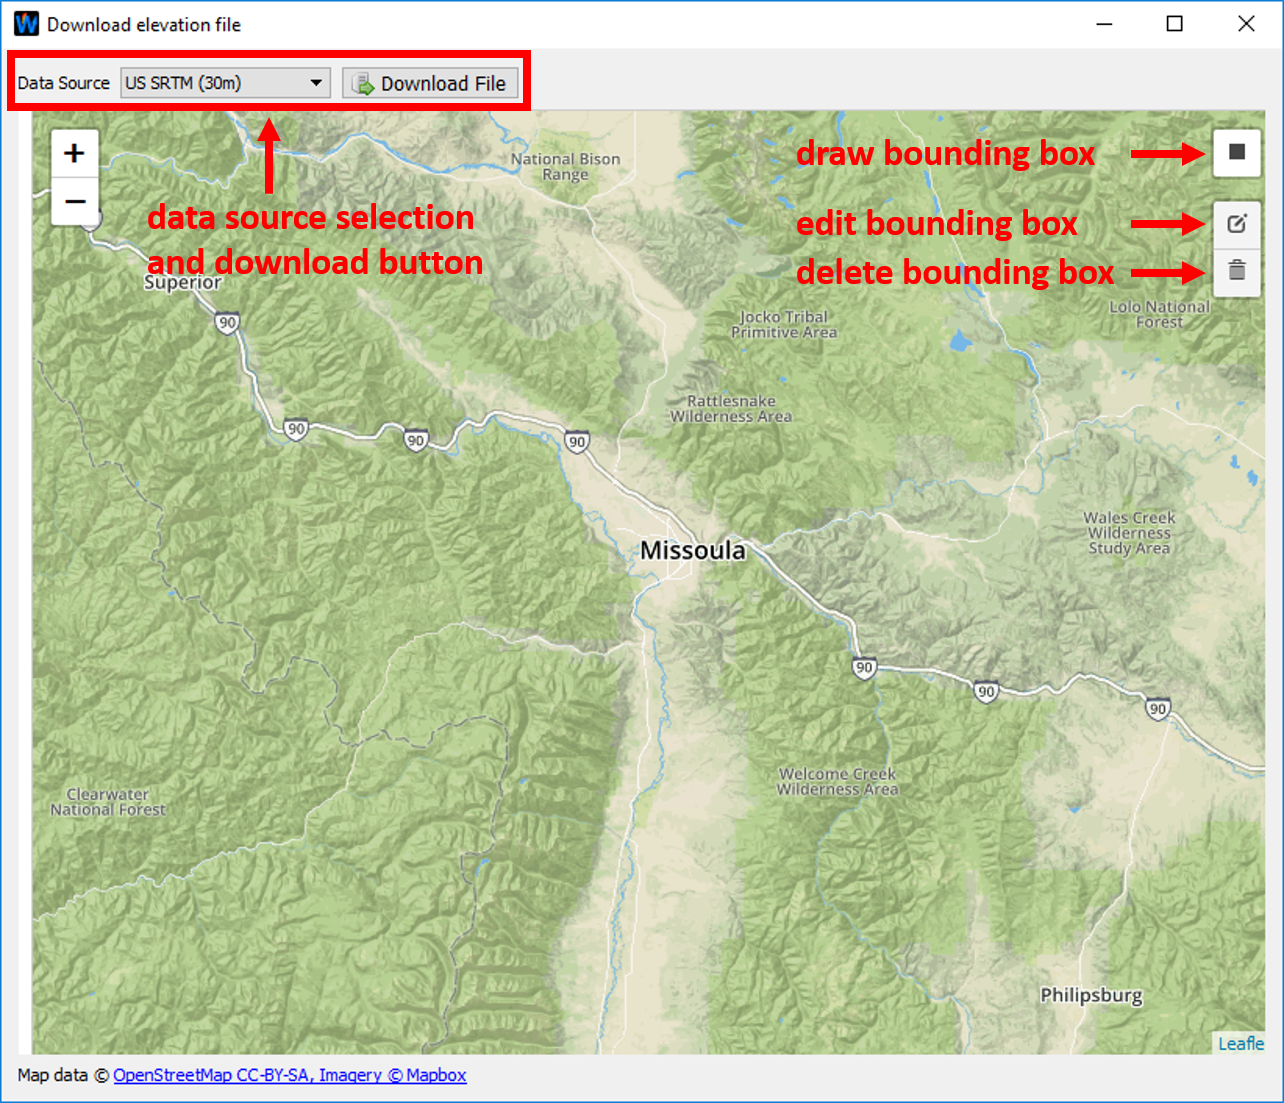
\includegraphics[scale=0.75]{dem_download_1}
\end{figure}

\subsection*{Defining Your Simulation Area}

There are three ways to define the area you want to download. 
\begin{enumerate}
\item Click the \textit{Draw bounding box} button in the upper right corner of the graphics window. Draw a box on the map bounding the area that you want to simulate. A transparent blue box will be drawn in the graphics window showing the area you've defined. 
\item Use the \textit{Point and Radius} method. Enter a latitude and longitude in decimal degrees specifying the center of the domain and a radius in miles specifying the distance from the center of the domain to the bounding box edge.
\item Specify the \textit{Bounding Box Coordinates} directly by entering the north and south latitudes and the east and west longitudes in decimal degrees that define your bounding box.
\end{enumerate}
The bounding box coordinates will be displyed in the \textit{Bounding Box Coordinates} text boxes at the bottom of the graphics window once a bounding box has been defined by any method. These coordinates can be edited to change the size of the bounding box. The blue box on the map will update when the \textit{Bounding Box Coordinates} are edited. If a bounding box has been already defined, clicking on the \textit{Draw bounding box} button will delete it.

\subsection*{Elevation Data Source}

There are 3 possible on-line data sets to download elevation data from.  These are listed in the \textit{Data Source} drop-down box at the top left of the graphics window.  The main difference between these data sets is the spatial resolution and extent.  The table below briefly describes these differences.  You should be sure to choose a data set that covers your simulation area.

\begin{center}
    \begin{tabular}{| l | l | p{1.75in} | p{1.8in} |}
    \hline
    Data set name & Resolution & Spatial Extent & Description \\ \hline

    WORLD SRTM & 30 meters & Between approximately -60 and +60 latitude &
    Data from the Shuttle Radar Tomography Mission (SRTM) \\ \hline

    WORLD GMTED & 250 meters & Between approximately -60 and +85 latitude &
    Global Multi-resolution Terrain Elevation Data 2010 (GMTED 2010) \\ \hline

    Landscape (LCP) & 30 meters & Contiguous US, Hawaii, PR, Southern Alaska &
    FARSITE Landscape files including vegetation information \\ \hline
\end{tabular}
\end{center}


\section*{Download The File}
Once you have defined your download area and selected the elevation data source, click the \textit{Download File} button at the top left of the graphics window to download the elevation file.  A window will open to allow you to specify a file name and location. The downloaded file will be a GeoTIFF file (*.tif) in best fit UTM projection using WGS84. After the file is successfully downloaded, you can close the Download elevation file window and the downloaded file will be automatically loaded into the main WindNinja window.


\end{document}
